\let\negmedspace\undefined
\let\negthickspace\undefined
\documentclass[journal]{IEEEtran}
\usepackage[a5paper, margin=10mm, onecolumn]{geometry}
%\usepackage{lmodern} % Ensure lmodern is loaded for pdflatex
\usepackage{tfrupee} % Include tfrupee package

\setlength{\headheight}{1cm} % Set the height of the header box
\setlength{\headsep}{0mm}     % Set the distance between the header box and the top of the text

\usepackage{gvv-book}
\usepackage{gvv}
\usepackage{cite}
\usepackage{amsmath,amssymb,amsfonts,amsthm}
\usepackage{amsmath}
\usepackage{algorithmic}
\usepackage{graphicx}
\usepackage{textcomp}
\usepackage{xcolor}
\usepackage{txfonts}
\usepackage{listings}
\usepackage{enumitem}
\usepackage{mathtools}
\usepackage{gensymb}
\usepackage{comment}
\usepackage[breaklinks=true]{hyperref}
\usepackage{tkz-euclide} 
\usepackage{listings}
% \usepackage{gvv}                                        
\def\inputGnumericTable{}                                 
\usepackage[latin1]{inputenc}                                
\usepackage{color}                                            
\usepackage{array}                                            
\usepackage{longtable}                                       
\usepackage{calc}                                             
\usepackage{multirow}                                         
\usepackage{hhline}                                           
\usepackage{ifthen}                                           
\usepackage{lscape}
\usepackage{circuitikz}
\tikzstyle{block} = [rectangle, draw, fill=blue!20, 
    text width=4em, text centered, rounded corners, minimum height=3em]
\tikzstyle{sum} = [draw, fill=blue!10, circle, minimum size=1cm, node distance=1.5cm]
\tikzstyle{input} = [coordinate]
\tikzstyle{output} = [coordinate]


\begin{document}

\bibliographystyle{IEEEtran}
\vspace{3cm}

\title{1.2.26}
\author{AI25BTECH11018-Hemanth Reddy}
 \maketitle
% \newpage
% \bigskip
{\let\newpage\relax\maketitle}

\renewcommand{\thefigure}{\theenumi}
\renewcommand{\thetable}{\theenumi}
\setlength{\intextsep}{10pt} % Space between text and floats


\numberwithin{equation}{enumi}
\numberwithin{figure}{enumi}
\renewcommand{\thetable}{\theenumi}

\textbf{Question:}\\

Rain is falling vertically with a speed of $35~ms^{-1}$. A woman rides a bicycle with a speed of $12~ms^{-1}$ in east to west direction. What is the direction in which she should hold her umbrella~?\\
\textbf{Solution:}\\

Velocity of rain $\overrightarrow{v}_{rain}=\myvec{0\\
-35}$\\
\vspace{0.7cm}
Velocity of woman $\overrightarrow{v}_{woman}=\myvec{-12\\0}$\\
The relative velocity of rain with respect to the woman is:$$\overrightarrow{v}_{rel}=\overrightarrow{v}_{rain}-\overrightarrow{v}_{woman}\\ = \myvec{0\\
-35}-\myvec{-12\\0}= \myvec{12\\-35}$$\\
 $$Let \quad 
\overrightarrow{a} = \myvec{1\\0}$$\\

Let $\theta$ be the angle with horizontal\\
\centering{$$\cos \theta= \frac{a^{T} v_{rel}}{||a||v_{rel}||}$$

$$\cos \theta= \frac{12}{37}$$
}

\begin{figure}
    \centering
    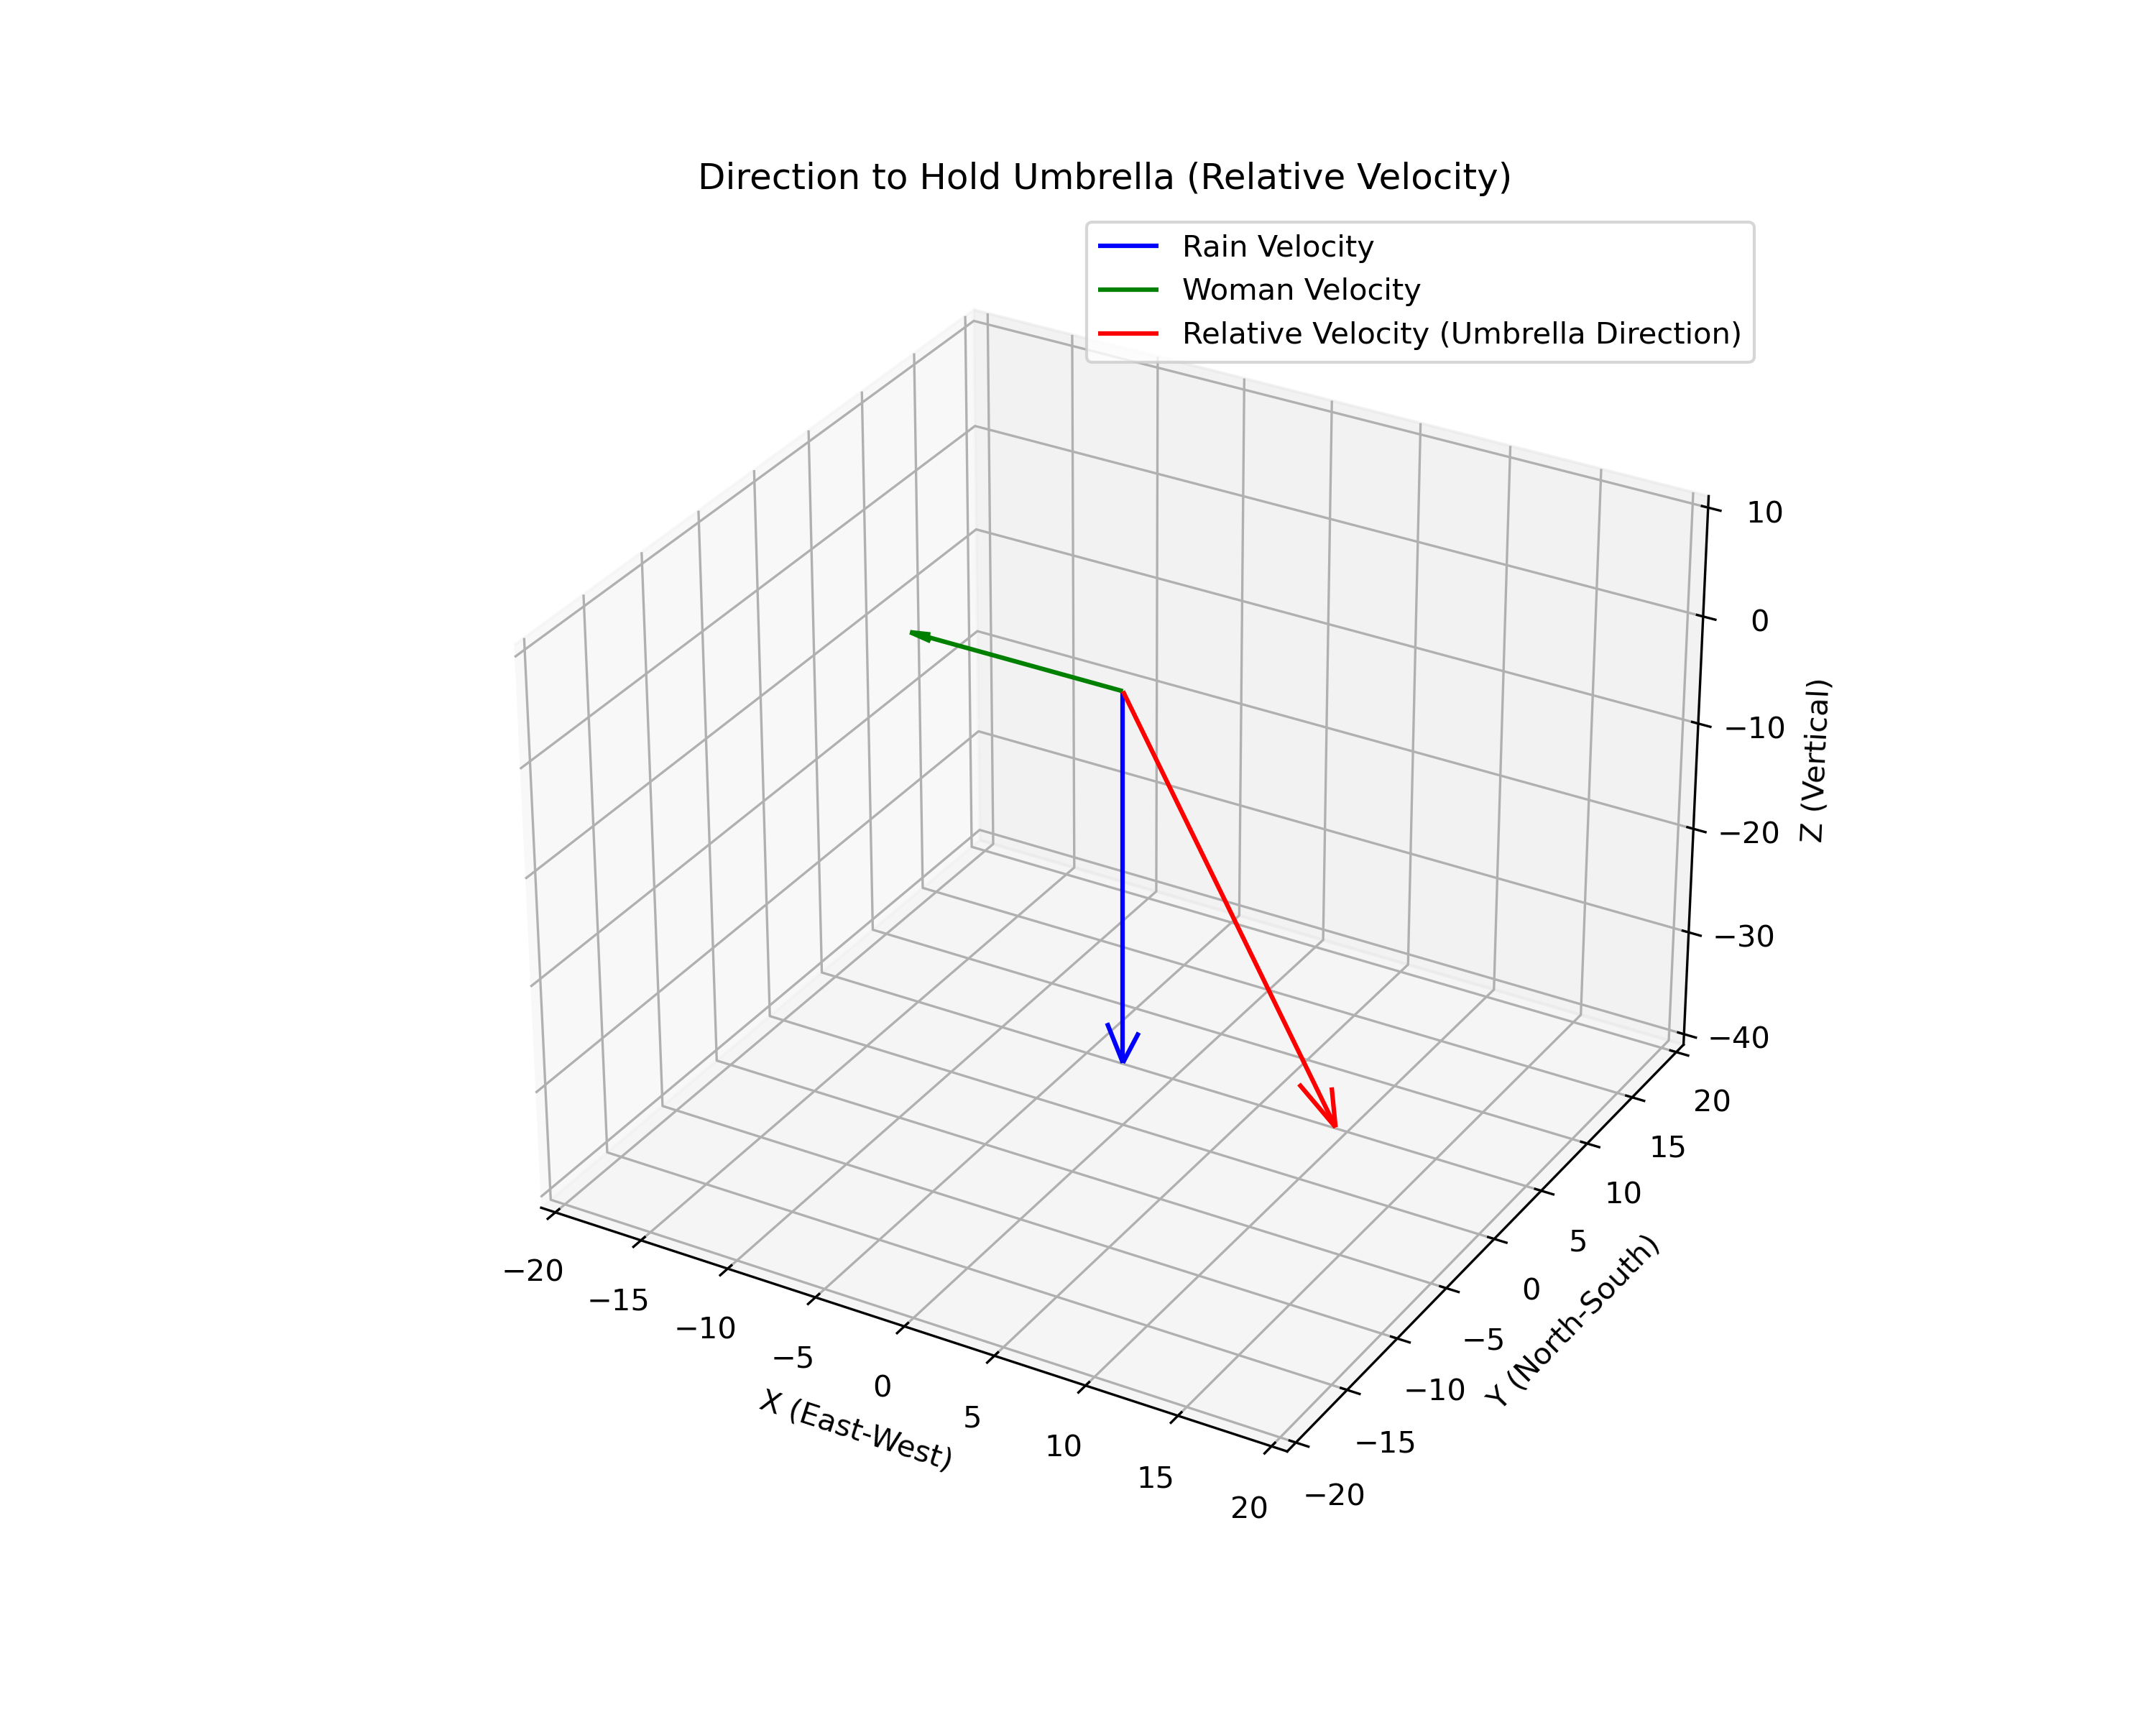
\includegraphics[width=0.8\columnwidth]{figs/fig.png}
    \caption{}
    \label{fig:placeholder}
\end{figure}






\end{document}